% Overview of the FEniCS(x) software
% Author: Julius Herb
% Based on a tikz template by Pavel Seda
% Sourcce: https://texample.net/tikz/examples/android/
\documentclass[tikz,border=2mm,convert={outfile=test.svg}]{standalone}

\usepackage{tikz}
\usetikzlibrary{arrows.meta}
\tikzset{%
  >={Latex[width=2mm,length=2mm]},
  % Specifications for style of nodes:
            base/.style = {rectangle, rounded corners, draw=black,
                           minimum width=4cm, minimum height=1cm,
                           text centered, font=\sffamily, align=center},
  dolfin/.style = {base, fill=blue!30},
       maths/.style = {base, fill=red!30},
    solution/.style = {base, fill=green!30},
         process/.style = {base, minimum width=2.5cm, fill=orange!15},
}
\begin{document}    
% Drawing part, node distance is 1.5 cm and every node
% is prefilled with white background
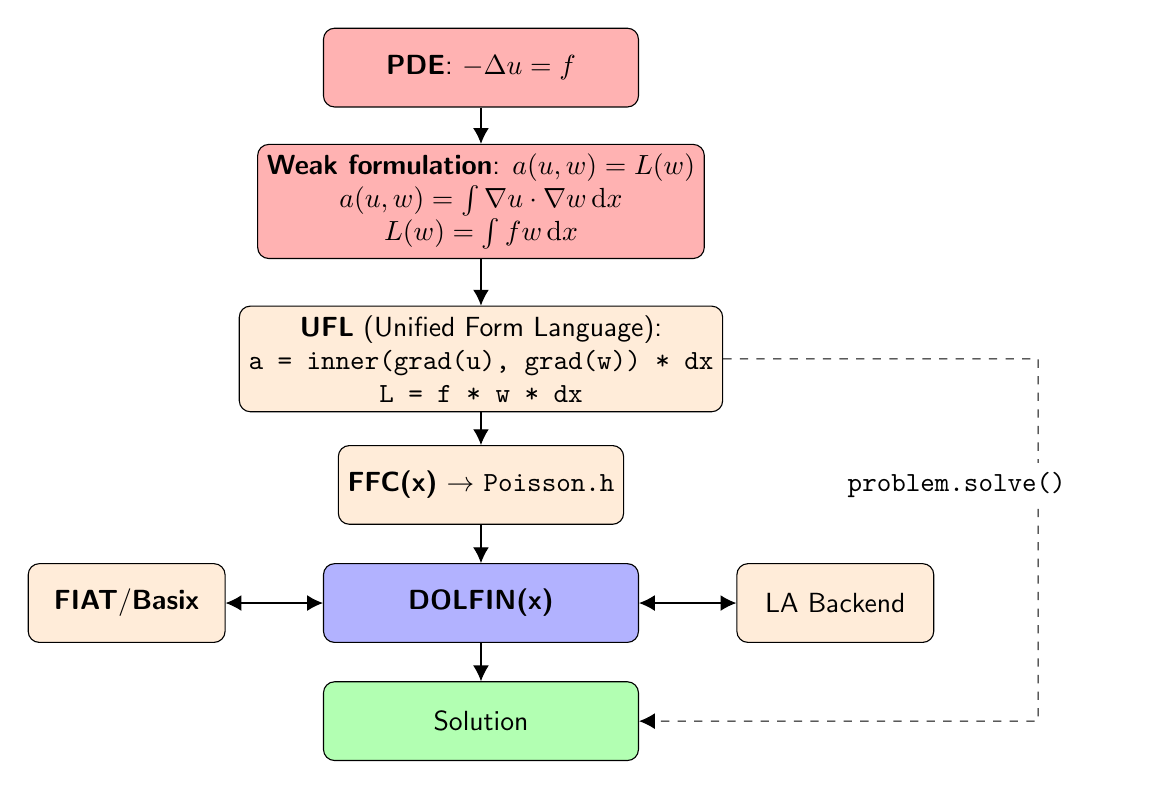
\begin{tikzpicture}[node distance=1.5cm,
  every node/.style={fill=white, font=\sffamily}, align=center]
% Specification of nodes (position, etc.)
\node (pde)             [maths]              {\textbf{PDE}: $-\Delta u = f$};
\node (weakform)     [maths, below of=pde, yshift=-2mm]          {\textbf{Weak formulation}: $a(u, w) = L(w)$ \\ $a(u, w) = \int \nabla u \cdot \nabla w \, \mathrm{d}x$ \\ $L(w) = \int f w \, \mathrm{d}x$};
\node (ufl)      [process, below of=weakform, yshift=-5mm]   {\textbf{UFL} (Unified Form Language): \\ \texttt{a = inner(grad(u), grad(w)) * dx} \\ \texttt{L = f * w * dx}};
\node (ffcx)     [process, below of=ufl, yshift=-1mm]   {\textbf{FFC(x)} $\rightarrow$ \texttt{Poisson.h}};
\node (dolfinx)      [dolfin, below of=ffcx, yshift=0mm]
                                                    {\textbf{DOLFIN(x)}};
\node (labackend)    [process, right of=dolfinx, xshift=3cm]
                                                            {LA Backend};
\node (basix)      [process, left of=dolfinx, xshift=-3cm]
                                                      {\textbf{FIAT}/\textbf{Basix}};
\node (solution) [solution, below of=dolfinx, yshift=0mm]
                                                  {Solution};     
% Specification of lines between nodes specified above
% with aditional nodes for description 
\draw[->]             (pde) -- (weakform);
\draw[->]     (weakform) -- (ufl);
\draw[->]      (ufl) -- (ffcx);
\draw[->]     (ffcx) -- (dolfinx);
\draw[<->]      (dolfinx) -- (basix);
\draw[<->]      (dolfinx) -- (labackend);
\draw[->]       (dolfinx) -- (solution);
\draw[->, dashed] (ufl.east) -- ++(4,0) -- ++(0,-2.6) -- ++(0,-2) --                
   node[xshift=1.5cm,yshift=3cm, text width=4cm]
   {\texttt{problem.solve()}}(solution.east);
\end{tikzpicture}
\end{document}

